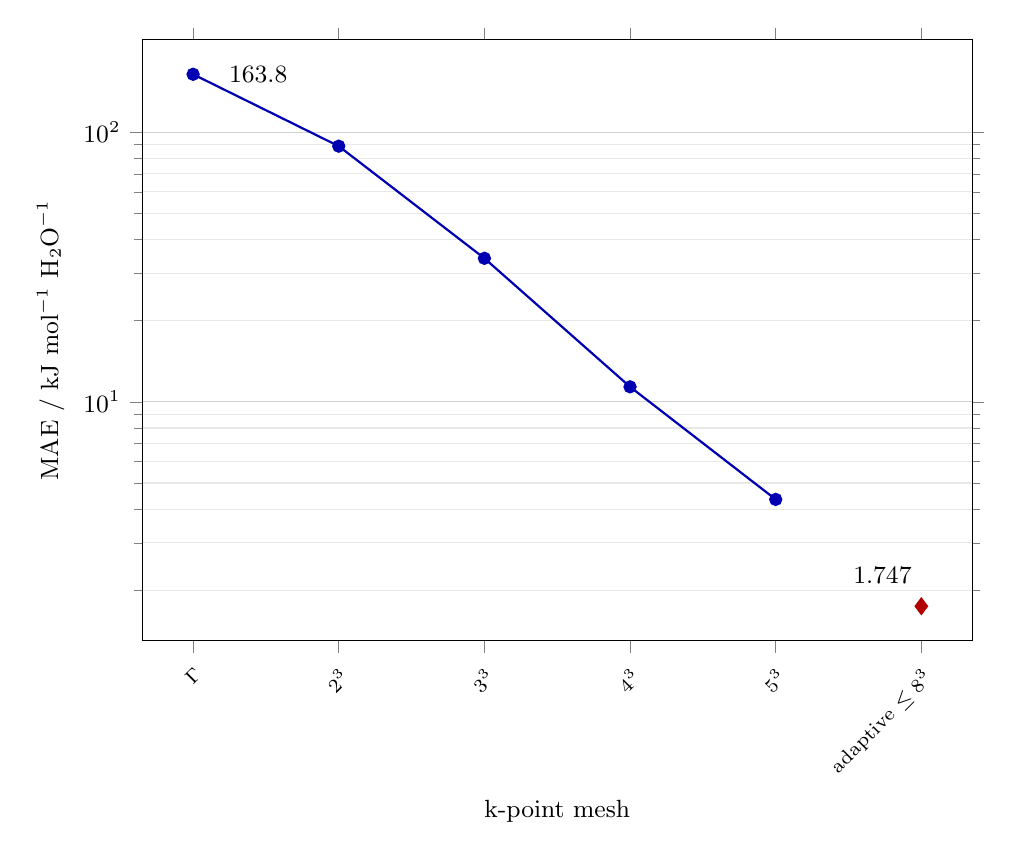
\begin{tikzpicture}
\begin{semilogyaxis}[
  width=\columnwidth,
  height=0.76\columnwidth,
  xmin=0.65,
  xmax=6.35,
  ymin=1.3,
  ymax=220,
  xtick={1,2,3,4,5,6},
  xticklabels={$\Gamma$,$2^3$,$3^3$,$4^3$,$5^3$,adaptive $\leq8^3$},
  x tick label style={rotate=45,anchor=north east,font=\scriptsize},
  y tick label style={font=\small},
  label style={font=\small},
  xlabel={k-point mesh},
  ylabel={MAE / kJ mol$^{-1}$ H$_2$O$^{-1}$},
  grid=both,
  xmajorgrids=false,
  major grid style={gray!35},
  minor grid style={gray!18},
  axis line style={black},
  tick align=outside,
  clip=false,
]
\addplot[
  blue!70!black,
  thick,
  mark=*,
  mark size=2pt,
] coordinates {
  (1,163.8344654)
  (2,88.6813751)
  (3,34.04848749)
  (4,11.36548083)
  (5,4.346421805)
};
\node[anchor=west,font=\small] at (axis cs:1.18,163.8344654) {163.8};
\addplot[
  red!70!black,
  only marks,
  mark=diamond*,
  mark size=3pt,
] coordinates {(6,1.746596161)};
\node[anchor=south east,font=\small] at (axis cs:6.0,1.956187701) {1.747};
\end{semilogyaxis}
\end{tikzpicture}
